% !TeX root = ../main.tex
\section{Lazy evaluation}

Up to now we've mostly asked ``what does this program compute?''. This section asks a
narrower but surprisingly consequential question: \emph{when} does an argument actually
get computed? Two languages can agree completely on what a program means and still
disagree on when the work happens, and that disagreement has real consequences for
what programs you can even write, not just how fast they run.

\subsection{eager vs. lazy, one more time}

Recall the call-by-value vs.\ call-by-name distinction: call-by-value evaluates an
argument before it's substituted into the function body, call-by-name substitutes the
unevaluated expression and re-evaluates it every time it's used. Eager (strict)
evaluation is the call-by-value discipline generalized to a whole language: every
subexpression is evaluated as soon as it's bound, full stop. Lazy evaluation is the
opposite discipline: an expression is not evaluated until (and unless) its value is
actually demanded.

This sounds like a small scheduling detail, but it changes what's even expressible.
Under eager evaluation, this Haskell-looking definition would loop forever before you
ever got a single element out of it:
\begin{lstlisting}[language=Haskell]
ones :: [Int]
ones = 1 : ones
\end{lstlisting}
Under lazy evaluation, it's a perfectly good infinite list, and \texttt{take 3 ones}
gives you \texttt{[1,1,1]} without ever trying to build the whole thing. Laziness
doesn't just delay work, it makes some values definable that couldn't be defined at all
under an eager discipline, because ``fully evaluate this'' would never terminate.

\begin{remark}
Call-by-name and call-by-value are about \emph{when an argument is substituted and
evaluated}. Eager and lazy evaluation are the same idea promoted to the level of an
entire language's evaluation strategy: does \emph{every} construct (let-bindings, data
constructors, function arguments) default to evaluate-immediately or
evaluate-on-demand?
\end{remark}

\subsection{call-by-need: call-by-name plus a memory}

Naive call-by-name has an obvious inefficiency: if an argument is used three times in
the function body, and it's re-substituted (and re-evaluated) at each use site, you do
the same work three times. \textbf{Call-by-need} fixes exactly this. It's call-by-name
with one addition: the first time an argument's value is demanded, the result is
\emph{cached}, and every subsequent use just reads the cached value instead of
recomputing it. This caching is called \textbf{memoization}, and it's the mechanism
that makes lazy evaluation, as actually implemented (in Haskell, in Miranda before it),
efficient enough to be a language's default strategy rather than a curiosity.

\begin{definition}[Thunk]
A \textbf{thunk} is a suspended, unevaluated computation packaged together with
everything it needs to run later: the expression to evaluate, plus the environment
(the bindings for its free variables) it should evaluate in. A thunk starts in an
\textsc{Unevaluated} state; the first time it is \textbf{forced} (its value is
demanded), it runs the suspended computation, overwrites itself with the result, and
switches to an \textsc{Evaluated} state so that every later force just returns the
cached value directly.
\end{definition}

Concretely, you can picture a thunk as a small mutable record:
\begin{lstlisting}[language=C]
typedef enum { UNEVALUATED, EVALUATED } ThunkState;

typedef struct Thunk {
    ThunkState state;
    /* if UNEVALUATED: */
    Expr       *expr;     /* the suspended expression */
    Env        *env;      /* captured environment, for free variables in expr */
    /* if EVALUATED: */
    Value      *value;    /* cached result, filled in the first time we force it */
} Thunk;

Value *force(Thunk *t) {
    if (t->state == UNEVALUATED) {
        t->value = eval(t->expr, t->env);   /* do the work, once */
        t->state = EVALUATED;               /* remember we did it */
    }
    return t->value;                        /* cheap from here on */
}
\end{lstlisting}
Every argument that's passed under call-by-need is really one of these records, not a
raw value. \texttt{force} is the single choke point: it's called every time something
actually needs to look inside the value (to pattern-match on it, print it, add it to
a number, \ldots), and it's the \texttt{if} check that turns re-evaluation into a cache
hit on every use after the first.

\begin{example}[Tracing a thunk being forced twice]
Suppose we bind \texttt{x = expensive(10)} where \texttt{expensive} is some slow
computation, under call-by-need, and then use \texttt{x} twice, in \texttt{x + x}.
\begin{enumerate}
  \item Binding \texttt{x} allocates a thunk in state \textsc{Unevaluated}, holding
        the expression \texttt{expensive(10)} and the current environment. No work
        has happened yet.
  \item Evaluating \texttt{x + x} needs the left \texttt{x}: we call
        \texttt{force(x)}. State is \textsc{Unevaluated}, so we actually run
        \texttt{expensive(10)}, get (say) \texttt{42}, overwrite the thunk with
        state \textsc{Evaluated} and value \texttt{42}.
  \item Evaluating the right \texttt{x} calls \texttt{force(x)} again. State is now
        \textsc{Evaluated}, so we skip straight to returning \texttt{42}. No
        recomputation.
\end{enumerate}
Total number of times \texttt{expensive} actually runs: one. That's the entire payoff
of call-by-need over plain call-by-name.
\end{example}

\subsection{weak head normal form}

Laziness means values are evaluated ``just enough'', but just enough for what,
exactly? The standard notion is \textbf{weak head normal form} (WHNF): an expression is
in WHNF once we know its outermost constructor (or, for a function, that it's a lambda
ready to be applied), \emph{without} having necessarily evaluated anything inside that
constructor.

For example, \texttt{1 : ones} (the infinite list from earlier) is in WHNF the moment
we know it's a cons cell with head \texttt{1}; the tail \texttt{ones} stays an
unevaluated thunk until something asks for it specifically. This is exactly why the
infinite list works at all: nothing ever demands the whole structure at once, each
\texttt{take} or pattern-match only forces one layer, one thunk, at a time.

\begin{example}[Self-referential infinite Fibonacci list]
\begin{lstlisting}[language=Haskell]
fibs :: [Integer]
fibs = 0 : 1 : zipWith (+) fibs (tail fibs)

-- take 10 fibs  ==>  [0,1,1,2,3,5,8,13,21,34]
\end{lstlisting}
This definition is self-referential: \texttt{fibs} is defined in terms of \texttt{fibs}.
Under eager evaluation this is nonsense (you can't compute \texttt{fibs} before you've
computed \texttt{fibs}). Under lazy evaluation, it works because each cons cell only
needs the previous cells to already be in WHNF, not fully evaluated, and \texttt{zipWith}
only ever forces one thunk ahead of where the consumer has gotten to. Tracing the third
element: \texttt{zipWith (+) fibs (tail fibs)}'s third element is
\texttt{fibs!!1 + fibs!!2}, which needs \texttt{fibs!!2}, which is itself defined by
the same zip one position earlier, and so on, bottoming out at the two literal
\texttt{0} and \texttt{1} thunks that started the list. Each position is computed once
and memoized, so this runs in linear time overall, not exponential.
\end{example}

\subsection{the catch: space leaks}

Laziness's classic gotcha is the \textbf{space leak}: instead of doing a computation as
you go, you build up a huge chain of unevaluated thunks, and pay for all of them at
once, later, plus the memory to hold the chain in the meantime.

The textbook example is \texttt{foldl} over a large list:
\begin{lstlisting}[language=Haskell]
foldl (+) 0 [1..1000000]
\end{lstlisting}
Under lazy evaluation, \texttt{foldl} does \emph{not} compute \texttt{0+1}, then
\texttt{1+2}, and so on as it walks the list. It builds up a thunk:
\[
  \big(\ldots((0+1)+2)+3\ldots+1000000\big)
\]
without ever forcing any of the additions, because nothing demanded the accumulator's
value along the way, only its ``shape'' (a thunk) was needed to keep folding. By the
time you finally force the result, you have a chain of a million nested unevaluated
additions sitting on the heap, and forcing it can blow the stack.

The fix is \texttt{foldl'}, the strict left fold, which forces the accumulator to WHNF
at every step instead of letting it pile up:
\begin{lstlisting}[language=Haskell]
foldl' (+) 0 [1..1000000]
\end{lstlisting}
Same result, but the accumulator is a plain number at every step of the loop instead of
a growing thunk chain; constant extra memory instead of linear.

\begin{center}
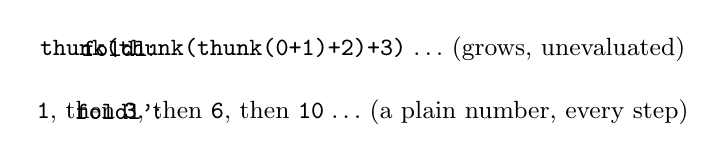
\begin{tikzpicture}[node distance=0.5cm]
  \node (a) [font=\small] {\texttt{foldl}:};
  \node (b) [right of=a, xshift=2.6cm, font=\small]
      {\texttt{thunk(thunk(thunk(0+1)+2)+3)}$\;\ldots$ (grows, unevaluated)};
  \node (c) [below of=a, yshift=-0.3cm, font=\small] {\texttt{foldl'}:};
  \node (d) [right of=c, xshift=2.6cm, font=\small]
      {\texttt{1}, then \texttt{3}, then \texttt{6}, then \texttt{10}$\;\ldots$ (a plain number, every step)};
\end{tikzpicture}
\end{center}

This is the trade-off in one sentence: laziness is simpler to reason about
compositionally and lets you write infinite/self-referential structures naturally, but
strictness is more predictable in space, because you know exactly when work happens
instead of deferring it into an invisible pile.

\subsection{strictness analysis, briefly}

Compilers that target lazy languages don't want to pay the thunk-allocation overhead
for every single binding if it's obviously going to be forced immediately anyway (say,
an argument that's used in a strict numeric operation on every code path). \textbf{Strictness
analysis} is a compile-time analysis that tries to prove ``this expression will
definitely be demanded, so it's safe to evaluate it eagerly instead of building a
thunk''. When it succeeds, you get the safety and elegance of a lazy language's
semantics with the performance of eager evaluation for the common cases, without the
programmer having to sprinkle strictness annotations everywhere by hand. GHC does this
routinely; it's a big part of why idiomatic Haskell doesn't leak thunks nearly as often
as the naive \texttt{foldl} example above.

\subsection{Exercises}
\begin{itemize}
  \item Trace by hand how many times \texttt{expensive(10)} actually runs under (a)
    call-by-name and (b) call-by-need, if \texttt{x = expensive(10)} is used four times
    in the function body. Justify both numbers using the thunk state machine above.
  \item Write out the thunk record (state, expression, environment) that would exist at
    the moment \texttt{take 3 (1 : ones)} has produced its first element but not yet
    touched the rest of the list.
  \item \texttt{fibs = 0 : 1 : zipWith (+) fibs (tail fibs)}: draw the chain of thunks
    that gets forced to compute the 4th element (index 3, value \texttt{2}), showing
    which earlier elements get reused from the cache rather than recomputed.
  \item Explain, in your own words, why \texttt{foldr (:) [] xs} does not have the same
    space-leak problem that \texttt{foldl (+) 0 xs} does, even though both are lazy.
  \item Think about it: could a strict (eager) language ever represent something like
    the infinite \texttt{fibs} list above without changing the language? What would you
    have to add (a special construct, a library type) to fake it?
  \item Some languages (Python generators, C\# \texttt{yield}, JavaScript generators)
    let you opt into a form of laziness on a per-value basis without making the whole
    language lazy by default. Compare this design to Haskell's ``lazy by default''
    stance: what do you gain and lose by making laziness opt-in instead of the default?
\end{itemize}
